\documentclass[a4paper]{beamer}

\title{Idealised GFD Models II}
\author{Tim Leslie}\institute{Breakaway Consulting Pty. Ltd.\\Climate Change Research Centre}

\newcommand {\framedgraphic}[2] {
    \begin{frame}{#1}
        \begin{center}
            
        \end{center}
    \end{frame}
}

\begin{document}

\begin{frame}
\titlepage
\begin{columns}
    \begin{column}{0.25\textwidth}
      
\includegraphics[keepaspectratio]{CC-BY-SA.png}
    \end{column}
    \begin{column}{0.75\textwidth}
      This work is licensed under a \href{http://creativecommons.org/licenses/by-sa/3.0/}{Creative Commons Attribution-ShareAlike 3.0 Unported License}. Copyright 2012 Tim Leslie.
    \end{column}
\end{columns}
\end{frame}

\begin{frame}{Ocean Modeling}
We would like to simulate the ocean to find out how it behaves. To do this we need to
\begin{itemize}
\item Write down equations to describe the physics involved
\item Solve these equations
\end{itemize}
\end{frame}


\begin{frame}{Numerically solving a differential equation}
Consider the D.E.
\begin{eqnarray}
\frac{d y}{d x} & = & x^2\\
y(1) & = & 1
\end{eqnarray}
Analytical techniques give
\begin{eqnarray}
y(x) & = & \frac{x^3 + 2}{3}
\end{eqnarray}
But what if we didn't have analysis?
\end{frame}

\begin{frame}{Numerical Solution}
Definition of the derivative
\begin{eqnarray}
f'(x) & = & \frac{f(x+\Delta x) - f(x)}{\Delta x}\\
f(x + \Delta x) & = & f(x) + f'(x)\Delta x
\end{eqnarray}
We can numerically solve our problem using different values of $\Delta x$
\begin{eqnarray}
f'(x) & = & x^2\\
f(1) & = & 1
\end{eqnarray}

\begin{tabular}{|r|c|c|c|c|c|}
\hline
$x=$  & 1 & 1.25   & 1.5   & 1.75  & 2.0\\
\hline
\hline
$\Delta x=1.00$          & 1 &        &       &       & 2\\
\hline
$\Delta x=0.50$          & 1 &        & 1.5 &         & 2.625\\
\hline
$\Delta x=0.25$          & 1 & 1.25   & 1.641 & 2.203 & 2.969\\
\hline
$\Delta x \rightarrow 0$ & 1 & 1.318  & 1.792 & 2.453 & 3.333\\
\hline
\end{tabular}
\end{frame}

\begin{frame}{Numerical integration}
\begin{itemize}
\item Given initial state, $f(t_0)$, and $f'(t)$ we can compute $f(t)$ into the future
\item We call this process \emph{numerical integration}
\item We can use numerical integration to solve the equations describing physical processes.
\end{itemize}
\end{frame}

\begin{frame}{QG Equations}
Recall the quasigeostropic equations over a horizontal layer.
\begin{eqnarray}
q_t & = & - \left(uq\right)_x - \left(vq\right)_y  -\frac{f_0}{H}\delta_z(e)+ A_2\frac{\nabla^4_Hp}{f_0}\\
q &    =   & \frac{\nabla^2_Hp}{f_0} + \beta(y - y_0) + \frac{f_0}{H}\delta_z(\eta)\\
(u, v) & = & \frac{1}{f_0}(-p_y, p_x)\\
\eta & = & \frac{(p_- - p_+)}{g^\prime}
\end{eqnarray}
\begin{itemize}
\item If we know $q$ (vorticity), we can compute $p$ (pressure)\\
\item If we know $q, p$ we can compute $q_t$\\
\item Therefore, if we know $q$ at a particular point in time, we can numerically integrate to find $q$ into the future.
\end{itemize}
\end{frame}

\begin{frame}{Control variables}
As well as the dynamic state variables $p, q$, the equations have two other types of variables
\begin{itemize}
\item Fixed control parameters ($f_0, \beta, H, A_2, g^\prime$)
\item Dynamic coupling variables ($e$)
\end{itemize}
By adjusting these variables we can perform different experiments to investigate the nature of the system being modelled.
\end{frame}

\begin{frame}{Q-GCM}
We will now consider a complete model consisting of 5 components
\begin{itemize}
\item QG ocean
\item Ocean mixed layer
\item Wind stress
\item QG Atmosphere
\item Atmosphere mixed layer
\end{itemize}
Each component has state variables, control parameters and dynamic coupling variables.
\end{frame}

\begin{frame}{Component Coupling}
  \begin{center}
    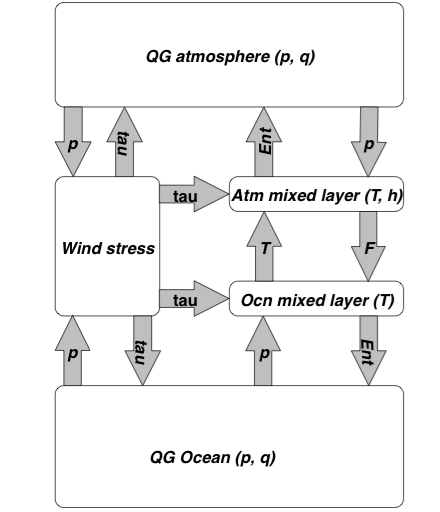
\includegraphics[width=\textwidth,height=0.8\textheight,keepaspectratio]{Q-GCM_Block_Diagram.png}
  \end{center}
\end{frame}


\begin{frame}{Running a Model}
\begin{itemize}
\item Choose values for control parameters
\item Set initial conditions of state variables
\item Numerically integrate model equations for a set period of time
\item Analyse output
\end{itemize}
\end{frame}

\begin{frame}{Model Output}
Models calculate two types of output:
\begin{itemize}
\item Prognostic quantities: The state variables use in the model calculation
\item Diagnostic quantities: Values derived from state variables, but not needed for the numerical integration itself
\end{itemize}
\end{frame}

\begin{frame}{Example Diagnostics}
Diagnostics let us investigate physical properties of the system being modelled.
\begin{itemize}
\item Average transport
\item Average kinetic energy
\item Max absolute velocity
\item Total convective heat transport
\item and many more...
\end{itemize}
\end{frame}

\begin{frame}{Summary}

\begin{itemize}
\item Climate models let us numerically integrate equations representing the physical world
\item Models are composed of multiple interacting components
\item Each component has controls parameters which can be adjusted to investigate different processes
\item Diagnostic output lets us obtain useful physical information from the model as it runs
\end{itemize}
\end{frame}

\end{document}
